{
    \subsection{Հարցումների ավտոմատ գեներացման համակարգ}\label{subsec:queryAggregation}
    Ծրագրային կոդի հատկությունների հարցումների համակարգի նպատակն է օգտագործողների համար հեշտացնել ծրագրերի վերլուծության
    գործընթացը: Այս նպատակին հասնելու համար մշակվել է հարցումների ավտոմատ գեներացման համակարգ:

    Ավտոմատ գեներացման համակարգի նպատակն է ավտոմատացնել հարցումների ստեղծման գործընթացը:
    Այն թույլ է տալիս օգտագործողներին առանց
    ինքնուրույն տվյալների բազայի հարցումներ գրելու՝ ստանալ անհրաժեշտ տեղեկություններ տվյալների բազայից:

    \begin{figure*}[t!]
        \centering
        \begin{subfigure}[t]{0.3\textwidth}
            \centering
            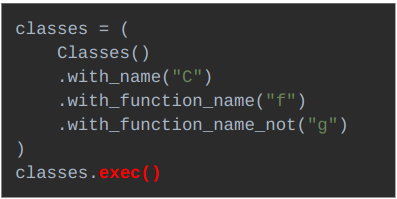
\includegraphics[height=1.2in]{pic11}
            \caption{}
            \label{fig:sub1}
        \end{subfigure}%
        ~
        \begin{subfigure}[t]{0.8\textwidth}
            \centering
            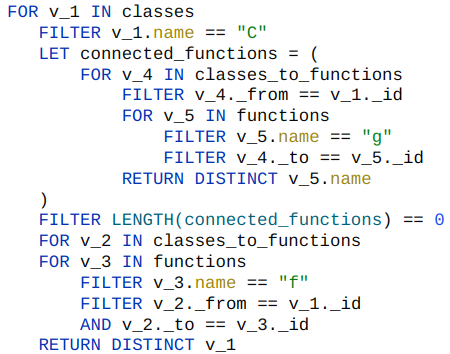
\includegraphics[height=3in]{pic12}
            \caption{}
            \label{fig:sub2}
        \end{subfigure}
        \caption{Հարցումների համակարգի հարցումների (a) և ավտոմատ կերպով գեներացված տվյալների բազայի հարցումների (b) օրինակ}
        \label{fig:figure11}
    \end{figure*}

    Այսպիսով, օգտագործողներին չի պահանջվի մշակել բարդ հարցումներ տվյալների բազայի համար:
    Փոխարենը, նրանք կկարողանան օգտագործով մշակված API-ը, ստանալ անհրաժեշտ տեղեկատվություն ծրագրի վերաբերյալ:

    Նկար \ref{fig:sub1}-ում ներկայացված է հարցումների համակարգի API-ի օգտագործմամբ մշակված հարցման օրինակ,
    իսկ Նկար \ref{fig:sub2}-ում հարցումների ավտոմատ գեներացման համակարգի կողմից գեներացված տվյալների բազայի հարցումը։
}